\chapter{归约}


\section{从最大匹配说起}

对于许多问题来说,寻求一个直接的解答、构造一个直接解决问题的算法是非常困难的。我们早已习惯通过变换问题的结构、挖掘问题的性质,在一个困难的问题中抽取出模型,
然后用已有的算法来解决,这就是问题与问题之间的归约。
在问题求解的过程中,归约使用的如此频繁,甚至很多时候我们都没有意识到自己实际上已经将一个问题归约成了另一个问题。问题与问题之间转化的过程
通常隐含了归约的过程。我们现在来看一个大家十分熟悉的问题:

\begin{prob}[二分图最大匹配, BIMATCH]
 给定二分图$G(X,Y,E)$,求$G$的一个最大匹配。$M$是$G$的匹配当且仅当$M\subseteq E$满足
 任意的$e_1, e_2 \in M$有$e_1\cap e_2 = \varnothing$。
\end{prob}

求解二分图最大匹配的一个有效算法是将它归约到网络最大流问题,如图 \ref{fig:match-to-flow} 所示。
二分图最大匹配的过程实际是一个算法,它接受二分图$G$作为输入,生成一个单位容量的流网络$G'$,然后求解$G'$的网络最大流,最大流的流量对应着最大匹配的数量,
而最大流中一些边的流量则对应着具体的匹配。


\begin{figure}[h]
 \center
 \begin{tikzpicture}
 \begin{scope}
  \node[vertex](l4) at (0, 0) {$d$};
  \node[vertex](l3) at (0, 1) {$c$};
  \node[vertex](l2) at (0, 2) {$b$};
  \node[vertex](l1) at (0, 3) {$a$};
  \node[vertex](r4) at (2, 0) {$d'$};
  \node[vertex](r3) at (2, 1) {$c'$};
  \node[vertex](r2) at (2, 2) {$b'$};
  \node[vertex](r1) at (2, 3) {$a'$};
  \path[-]
    (l1) edge (r1)
    (l1) edge (r2)
    (l2) edge (r1)
    (l2) edge (r3)
    (l2) edge (r4)
    (l3) edge (r1)
    (l3) edge (r3)
    (l4) edge (r4)
;
  \path[-, line width=1pt]
    (l1) edge (r2)
    (l2) edge (r1)
    (l3) edge (r3)
    (l4) edge (r4)
;
 \end{scope}

 \begin{scope}[xshift=6cm]
  \node[vertex](l4) at (0, 0) {$d$};
  \node[vertex](l3) at (0, 1) {$c$};
  \node[vertex](l2) at (0, 2) {$b$};
  \node[vertex](l1) at (0, 3) {$a$};
  \node[vertex](r4) at (2, 0) {$d'$};
  \node[vertex](r3) at (2, 1) {$c'$};
  \node[vertex](r2) at (2, 2) {$b'$};
  \node[vertex](r1) at (2, 3) {$a'$};
  \node[vertex](s) at (-1.5, 1.5) {$s$};
  \node[vertex](t) at (3.5, 1.5) {$t$};
  \path[-stealth]
   (s) edge (l1) (s) edge (l2) (s) edge (l3) (s) edge (l4)
   (r1) edge (t) (r2) edge (t) (r3) edge (t) (r4) edge (t)
;
  \path[-stealth]
    (l1) edge (r1)
    (l1) edge (r2)
    (l2) edge (r1)
    (l2) edge (r3)
    (l2) edge (r4)
    (l3) edge (r1)
    (l3) edge (r3)
    (l4) edge (r4)
;
  \path[-stealth, line width=1pt]
    (l1) edge (r2)
    (l2) edge (r1)
    (l3) edge (r3)
    (l4) edge (r4)
    (s) edge (l1) (s) edge (l2) (s) edge (l3) (s) edge (l4)
    (r1) edge (t) (r2) edge (t) (r3) edge (t) (r4) edge (t)
;
 \end{scope}

 \end{tikzpicture}
 \caption{二分图最大匹配到网络最大流的归约}
 \label{fig:match-to-flow}
\end{figure}

在上述归约中,如果二分图$G$包含$V$个结点和$E$条边,我们构造的流网络就有
$V+2$个结点和$E+2V$条边,归约前后问题的规模几乎是相同的。
然而这并不总是成立,归约前后问题的规模可能有很大的差别,
甚至会有指数级的增长(例如直接将二分图匹配问题归约到DNF-SAT)。 % maybe we can use another example
Dinic算法在求解这类具有特殊结构的网络流问题时有$O(\sqrt{V} E)$的时间复杂度,因此这个归约不仅很简洁,而且能够很高效地求解。

这个例子给了我们一些关于归约的启发:归约在大多数时候意味着用一个更通用的算法,来解决一个相对简单的问题。
我们构造了一个非常特殊的流网络求解了二分图匹配问题,而网络流所能解决问题的范畴则远远不止于此。
顺着这个思路,我们可以把二分图匹配的问题,乃至一般图匹配问题归约到一个更加一般的问题:

\begin{prob}[最大团, Clique]
给定有向图$G(V,E)$,求$G$中最大的点集$C\subseteq V$,满足对于任意的$u\neq v \in C$, $\{u, v\} \in E$。
每个满足条件的点集都是一个团,其中最大的则称为图的最大团。
\end{prob}

现在我们把二分图匹配归约到Clique,从$G(X, Y, E)$出发构造图$G'(V',E')$:令$V'$为$G$的边集$E$,
对于$G$中的每对边$e_1, e_2 \in E$,如果$e_1 \cap e_2 = \varnothing$,我们就将$\{e_1, e_2\}$添加到$E'$中。
这样$G'$中的每个团都对应$G$中的一个匹配,而$G$中的每一个匹配也对应$G'$中的一个团,因此
求解$G'$中的最大团,就能得到$G$中的最大匹配,如图 \ref{fig:match-to-clique} 所示。

\begin{figure}[h]
 \center
 \begin{tikzpicture}
 \begin{scope}
  \node[vertex](l4) at (0, 0) {$d$};
  \node[vertex](l3) at (0, 1) {$c$};
  \node[vertex](l2) at (0, 2) {$b$};
  \node[vertex](l1) at (0, 3) {$a$};
  \node[vertex](r4) at (2, 0) {$d'$};
  \node[vertex](r3) at (2, 1) {$c'$};
  \node[vertex](r2) at (2, 2) {$b'$};
  \node[vertex](r1) at (2, 3) {$a'$};
  \path[-]
    (l1) edge (r1)
    (l1) edge (r2)
    (l2) edge (r1)
    (l2) edge (r3)
    (l2) edge (r4)
    (l3) edge (r1)
    (l3) edge (r3)
    (l4) edge (r4)
;
  \path[-, line width=1pt]
    (l1) edge (r2)
    (l2) edge (r1)
    (l3) edge (r3)
    (l4) edge (r4)
;
 \end{scope}

 \begin{scope}[xshift=6cm]
  \node[vertex](e1) at (-1, 2) {$aa'$};
  \node[vertex, line width=1pt](e2) at (-1, 1) {$ab'$};
  \node[vertex, line width=1pt](e3) at (1, 0) {$ba'$};
  \node[vertex](e4) at (0, 3) {$bc'$};
  \node[vertex](e5) at (0, 0) {$bd'$};
  \node[vertex](e6) at (2, 1) {$ca'$};
  \node[vertex, line width=1pt](e7) at (2, 2) {$cc'$};
  \node[vertex, line width=1pt](e8) at (1, 3) {$dd'$};
  \path[-]
   (e1) edge (e4) (e1) edge (e5) (e1) edge (e7) (e1) edge (e8)
   (e2) edge (e3) (e2) edge (e4) (e2) edge (e5) (e2) edge (e6) (e2) edge (e7) (e2) edge (e8)
   (e3) edge (e6) (e3) edge (e7) (e3) edge (e8)
   (e4) edge (e8)
   (e5) edge (e6) (e5) edge (e7)
   (e6) edge (e8)
   (e7) edge (e8)
;
  \path[-, line width=1pt]
    (e2) edge (e3) (e2) edge (e7) (e2) edge (e8)
    (e3) edge (e7) (e3) edge (e8)
    (e7) edge (e8)
;
 \end{scope}

 \end{tikzpicture}
 \caption{二分图最大匹配到最大团的归约}
 \label{fig:match-to-clique}
\end{figure}

我们来把$G(X,Y,E)$的最大匹配归约到网络流和归约到Clique进行一些对比。
归约到Clique时所创建的图有$E$个结点和$O(V^2)$条边,我们看到,问题的规模已经呈现出了平方级的增长(尤其是在$G$很稀疏的情况下);
此外,Clique还是一个NP-完全问题,目前还没有任何一个算法能高效地解决它。尽管在实际求解时,由最大匹配问题归约而来的实例具有其特殊性,
一些好的solver可能有较好的效率(甚至可能总是能够在多项式时间内给出结果),
但总体而言,把最大匹配归约到Clique是正确的,但并没有给我们解决问题带来很大的帮助。
因此,我们希望理想的归约能有以下特性:

\begin{enumerate}
 \item 存在高效的算法实现归约过程,以及结果的转换。在前面的例子中,这样的转换算法都是十分朴素的,但在更复杂的问题中,归约过程本身就可能非常复杂。
 \item 归约后的问题存在高效的算法。除非我们待解决的问题是一个难问题,我们一般都希望归约后的问题能在多项式时间内解决。
 \item 归约后问题的规模在可求解的范围。
\end{enumerate}

\section{不同形式的归约}

之前我们展示的是归约中最常见,也是最简单的形式,如图 \ref{fig:reduction-show} 所示。
为了求解问题A,我们使用一个算法将A问题的输入转换为B问题的输入,求解B问题后再将B问题的输出转换为A问题的输出。
这种类型的归约通常能够找到两个问题实例之间的对应关系(例如一个二分图的某个匹配对应了某个流网络中的一个可行流,或是某个图中的一个团)。

\begin{figure}[h]
 \center
 \begin{tikzpicture}
  \matrix (m) [matrix of nodes,row sep=1.5em,column sep=1.5em,minimum width=1em]
  {
     问题A输入 &  输入转换  &  输出转换   & 问题A输出 \\
               & 问题B输入 &           & \\
               & 问题B算法 & 问题B输出 & \\
  };
  \path[-stealth]
    (m-1-1) edge (m-1-2) (m-1-3) edge (m-1-4)
    (m-1-2) edge (m-2-2)
    (m-2-2) edge (m-3-2)
    (m-3-2) edge (m-3-3) (m-3-3) edge (m-1-3)
;
  \node (thebox) [rectangle, draw=black, inner sep=1em, fit = (m-1-2) (m-3-3)] {};
 \end{tikzpicture}
 \caption{基本归约示意图}
 \label{fig:reduction-show}
\end{figure}

很多时候,我们寻找归约仅仅是为了改变问题的结构。难以直接求解的问题稍作改变,有时就变得容易,
下面的序列查询就是这样的例子:

\begin{prob}[序列查询]
 给出一列数字$A_1, A_2, \ldots A_n$和若干个查询,第$i$个查询$(x_i,y_i)$需要求出
 子序列$A_{x_i}, A_{x_{i+1}}, \ldots, A_{y_i}$中所有数字的和,但相同的数字只计算一次。
 例如序列$1, 10, 10, 1$的查询结果为$12$。
\end{prob}

试图直接解决这个问题是较为困难的。如果用朴素的算法,每次查询的时间复杂度将达到$O(n\log n)$。
当我们试图用数据结构优化这个查询时也遇到了困难:一个大区间的查询结果难以直接写成小区间查询结果的递推关系。
这个问题的归约实际是将问题作了适当的改写,将``不重复的数字''用数量刻画出来。引入辅助函数
$$B_i = 
\begin{cases}
 -1 & \textrm{$i$是$B_i$首次出现的位置} \\
 \displaystyle\argmax_{j < i} A_j = B_i & \textrm{否则.} \\
\end{cases}
$$
$B_i$的含义是每个数字在数列中上一次出现的位置。对于查询$(x, y)$中的某个数$A_i$,我们都查看它上一次出现的位置,
如果$B_i\geq x$,说明$A_i$这个数字已经在$A_x,A_{x+1}\ldots,A_{i-1}$中已经出现过,不再需要重复计算。因此,查询$(x,y)$被转化为求
$$
\sum_{t\in T} A_t, \textrm{其中\,}T = \{i ~|~ x \leq i \leq y\textrm{且\,} B_i < x_i \}.
$$
如果把序列中的每一个数字看作是二维平面上的一个点$(i, B_i)$,则一次查询$(x, y)$就被归约成求
矩形$(x, 0)-(y, B_x - 1)$中所有点$A_i$数值的和,而这是一个相对容易解决的经典问题,可以在$O(\log^2n)$的时间内获得查询结果。


这种类型的归约还是复杂性理论证明中的一个基本手段。例如,我们想要检查Clique这一问题的难度。显然$\mathrm{Clique}\in\mathrm{NP}$。
我们已知SAT问题是NP-完全的,如果我们能在多项式时间内,将一个SAT问题的输入$C$转换成一个最大团问题的输入$G$,并且$G$存在大小为$k$的团当且仅当SAT问题可被满足,
我们就能得出``Clique问题至少和SAT问题一样难''的结论。如果存在这样的归约,Clique就是NP-完全的。

\begin{prob}[最大权闭包, Closure]
 
\end{prob}

图 \ref{fig:reduction-show} 中的方框可以重复许多次,

%将最大权闭包归约到最小割。

%子树查询变为区间查询。

%GSS2中查询的归约。

%区间询问。

\section{归约到CNF-SAT问题}

CNF-SAT问题(后简称为SAT问题)是一类十分重要的基本问题,其问题描述如下:

\begin{prob}[合取范式可满足性, CNF-SAT, SAT]
 给定一个合取范式(CNF)表示的逻辑公式$C = C_1 \land C_2 \land \ldots \land C_n$,其中每一个子句(clause) $C_i$都是
 若干变量$x_i$或$\neg x_i$的析取(即或运算连接的)。求每个变量的一个赋值($T$或$F$),使$C$的值为真。例如
 $$(x_1)\land(\neg x_1 \lor x_2)\land(\neg x_2 \lor x_3)$$
 是可满足的,令$x_1=x_2=x_3=T$即可。
\end{prob}

SAT问题在计算机科学中有着十分重要的地位。对于每一个子句$C_i$中变量的个数不超过2的情况,2-SAT存在十分高效的算法;
但如果仅仅将这个限制放宽为$C_i$中变量个数不超过3,该问题就成为了NP-完全问题,这意味着所有NP问题都可以在多项式时间内归约到
3-SAT,SAT是最早被证明的NP-完全问题。

\begin{prob}[2-SAT]
 在SAT问题中,限制每个子句中包含的变量个数不超过2。不失一般性,我们假设每个子句都是$a\lor b (a \neq b)$的形式,其中$a, b$是变量$x_i$或$x_i$的取反$\neg x_i$。
\end{prob}

解决2-SAT问题的突破口是$(p\to q) = (\neg p \lor q)$。
我们可以将形如$a\lor b$的子句改写成蕴含的形式:$$(a\lor b) = (\neg a \to b) = (\neg b \to a) = (\neg a \to b) \land (\neg b \to a).$$
这样,2-SAT问题就被我们改写成了若干蕴含式的合取,此时问题的解决也十分明朗:建立有向图$G(V,E)$,其中$V$是由每个变量$x_i$和它的取反$\neg x_i$组成的,
而对于改写后的每一个蕴含式$a\to b$,都在图中添加一条由$a$指向$b$的边。
由于蕴含关系的传递性,若图中如果存在$x_i$到$\neg x_i$的路径,则说明2-SAT中包含矛盾,否则我们就可以依据蕴含关系求出2-SAT的一个解。
更进一步,因为$G$特殊的对称性(故意将一个析取式变换成了两个等价蕴含式的合取), $x_i$到$\neg x_i$存在路径总是意味着$\neg x_i$到$x_i$也存在路径,所以2-SAT最终被归约到有向图强连通分量问题的求解。
2-SAT适用于求解二元的约束关系,例如如下问题:
\begin{prob}[异或求解, XOR]
 给定非负整数权无向图$G(V, E, W)$,你需要为每一个结点$v$求一个整数标号$X_v$,使得对于每条边$\{u, v\}\in E$, $X_u \oplus X_v = W_{u,v}$。
 其中$\oplus$为按位异或运算。
\end{prob}

SAT是NP-完全问题,从目前的研究进展来看,设计一个算法能够高效地计算任意SAT问题的解是不现实的。但这并不意味着试图解决SAT问题的尝试完全是徒劳,其原因有二:
首先,SAT问题足够难,这样我们不仅可以把一些简单的问题归约到SAT,还可以将很多难问题归约到SAT,注意现实生活中的很多问题都是很困难的问题;
其次,SAT问题的形式十分特殊,问题的目标是求一个``满足约束条件的解'',而大量的现实问题都是要求在满足一定约束条件下的合法解。
许多NP-完全问题(例如哈密顿路问题)虽然能在多项式时间内与SAT互相归约,但把实际问题归约到它们却并不容易。
这些原因使归约到SAT成为了一类问题求解的标准途径。人们对SAT问题求解的需求增长,也刺激了对SAT问题求解的研究。
让我们高兴的是,即便SAT问题在理论上是十分困难的,但很多算法确实能非常高效地解决各种实际问题,
能够求解现实问题中数万个变量、数百万个子句的SAT问题实例,而且我们能从互联网上获取各种各样的SAT solver。
作为SAT solver的应用,我们首先介绍Exact Cover问题:

\begin{prob}[覆盖问题, Exact Cover]
 给定一个$n\times m$的01矩阵$A$,求一个行的集合$C\subseteq[n]$,满足对于任意的$j$, 
 $\sum_{i\in C} A_{i,j} = 1$。也就是说,我们要从$A$中取出若干行得到一个子矩阵,满足该子矩阵中每列恰好只有一个$1$。
 例如,若
 $$A = 
 \begin{pmatrix}
  0 & 0 & 0 & 1 & 0 & 1\\
  1 & 1 & 1 & 1 & 0 & 0\\
  1 & 0 & 1 & 0 & 1 & 0\\
  0 & 1 & 0 & 0 & 0 & 0\\
 \end{pmatrix},
 $$
 则$C=\{1, 3, 4\}$是一个合法的覆盖,而$\{1, 2, 4\}$则不是。
\end{prob}

% SPOJ 217
% 你在玩一个塔防小游戏,游戏在一张矩形地图上进行,地图上有4种格子,分别是防御塔、敌人、障碍和空地。你只能在游戏开始前调整防御塔的状态,虽然游戏开始以后敌人是不会动的,但你的目标是消灭所有的敌人,并保证防御塔之间不会误伤。

有些问题可以很自然地被归约到Exact Cover,例如下面提到的方块覆盖问题:

\begin{prob}[方块覆盖,Tetris]
给出一个$n\times n$的棋盘和一些给定的部件,棋盘上指定一些方格为空格。你需要用给定的部件不重叠地覆盖棋盘上所有的空格,每个部件最多只能使用一次。
\end{prob}

\begin{figure}[h]
 \center
 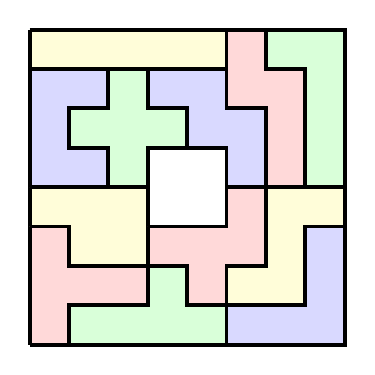
\begin{tikzpicture}[scale = 0.5]
  \draw[help lines] (0, 0) grid (8, 8);
  \draw[line width=0.5mm, fill=red!15] (0, 0) -- (1, 0) -- (1, 1) -- (3, 1) -- (3, 2) -- (1, 2) -- (1, 3) -- (0, 3) -- (0, 0);
  \draw[line width=0.5mm, fill=green!15] (1, 0) -- (5, 0) -- (5, 1) -- (4, 1) -- (4, 2) -- (3, 2) -- (3, 1) -- (1, 1) -- (1, 0);
  \draw[line width=0.5mm, fill=blue!15] (5, 0) -- (8, 0) -- (8, 3) -- (7, 3) -- (7, 1) -- (5, 1) -- (5, 0);
  \draw[line width=0.5mm, fill=yellow!15] (0, 3) -- (1, 3) -- (1, 2) -- (3, 2) -- (3, 4) -- (0, 4) -- (0, 3);
  \draw[line width=0.5mm, fill=red!15] (3, 2) -- (4, 2) -- (4, 1) -- (5, 1) -- (5, 2) -- (6, 2) -- (6, 4) -- (5, 4) -- (5, 3) -- (3, 3) -- (3, 2);
  \draw[line width=0.5mm, fill=yellow!15] (5, 1) -- (7, 1) -- (7, 3) -- (8, 3) -- (8, 4) -- (6, 4) -- (6, 2) -- (5, 2) -- (5, 1);
  \draw[line width=0.5mm, fill=blue!15] (0, 4) -- (2, 4) -- (2, 5) -- (1, 5) -- (1, 6) -- (2, 6) -- (2, 7) -- (0, 7) -- (0, 4);
  \draw[line width=0.5mm, fill=green!15] (2, 4) -- (3, 4) -- (3, 5) -- (4, 5) -- (4, 6) -- (3, 6) -- (3, 7) -- (2, 7) -- (2, 6) -- (1, 6) -- (1, 5) -- (2, 5) -- (2, 4);
  \draw[line width=0.5mm, fill=blue!15] (3, 6) -- (4, 6) -- (4, 5) -- (5, 5) -- (5, 4) -- (6, 4) -- (6, 6) -- (5, 6) -- (5, 7) -- (3, 7) -- (3, 6);
  \draw[line width=0.5mm, fill=red!15] (5, 6) -- (6, 6) -- (6, 4) -- (7, 4) -- (7, 7) -- (6, 7) -- (6, 8) -- (5, 8) -- (5, 6);
  \draw[line width=0.5mm, fill=green!15] (7, 4) -- (8, 4) -- (8, 8) -- (6, 8) -- (6, 7) -- (7, 7) -- (7, 4);
  \draw[line width=0.5mm, fill=yellow!15] (0, 8) -- (5, 8) -- (5, 7) -- (0, 7) -- (0, 8);
  \draw[line width=0.5mm, fill=gray!0] (3, 3) -- (3, 5) -- (5, 5) -- (5, 3) -- (3, 3);
 \end{tikzpicture}

 \caption{一个方块覆盖问题的实例}
 \label{fig:tetris}
\end{figure}

Exact Cover是一个NP-完全问题,使用Dancing Links数据结构的搜索配合一些启发策略是解决Exact Cover问题的通常手段。
为了充分利用SAT solver,我们现在将Exact Cover归约到SAT:我们为矩阵的每一行设置一个变量$x_i$,当$x_i=T$时,我们希望$i\in C$,相反当$x_i=F$时,$i\notin C$。
首先,我们希望矩阵中的每一列都被覆盖,因此对于每一列$j$,令$T_j = \{ i~|~ A_{i,j} = 1\}$, 则子句
$$\bigvee_{i \in T_j} x_i$$
代表了``第$j$列至少包含一个1''。
其次,我们希望每一列至多只有一个1。因此我们必须禁止某些行被同时选中,即对于每一对$(p,q)$,若第$p$行和第$q$行在同一列上有公共的1,我们还需要满足
$$\neg (x_p \land x_q) = (\neg x_p \lor \neg x_q).$$

将$n\times m$规模的Exact Cover归约到SAT问题后约有$O(m)$个$O(n)$大小的clause,以及$O(n^2)$个$O(1)$大小的clause,问题的整体规模并没有数量级上的提升,
这个归约可以用来解决很多问题,例如数独的求解。

\begin{figure}[h]
 \center

  \newcounter{row}
\newcounter{col}

\newcommand\setrow[9]{
  \setcounter{col}{1}
  \foreach \n in {#1, #2, #3, #4, #5, #6, #7, #8, #9} {
    \edef\x{\value{col} - 0.5}
    \edef\y{9.5 - \value{row}}
    \node[anchor=center] at (\x, \y) {\n};
    \stepcounter{col}
  }
  \stepcounter{row}
}

  \begin{tikzpicture}[scale=.5]

    \begin{scope}
      \draw (0, 0) grid (9, 9);
      \draw[very thick, scale=3] (0, 0) grid (3, 3);

      \setcounter{row}{1}
      \setrow { }{2}{ }  {5}{ }{1}  { }{9}{ }
      \setrow {8}{ }{ }  {2}{ }{3}  { }{ }{6}
      \setrow { }{3}{ }  { }{6}{ }  { }{7}{ }

      \setrow { }{ }{1}  { }{ }{ }  {6}{ }{ }
      \setrow {5}{4}{ }  { }{ }{ }  { }{1}{9}
      \setrow { }{ }{2}  { }{ }{ }  {7}{ }{ }

      \setrow { }{9}{ }  { }{3}{ }  { }{8}{ }
      \setrow {2}{ }{ }  {8}{ }{4}  { }{ }{7}
      \setrow { }{1}{ }  {9}{ }{7}  { }{6}{ }

      \node[anchor=center] at (4.5, -0.5) {一个数独问题};
    \end{scope}

    \begin{scope}[xshift=12cm]
      \draw (0, 0) grid (9, 9);
      \draw[very thick, scale=3] (0, 0) grid (3, 3);

      \setcounter{row}{1}
      \setrow { }{2}{ }  {5}{ }{1}  { }{9}{ }
      \setrow {8}{ }{ }  {2}{ }{3}  { }{ }{6}
      \setrow { }{3}{ }  { }{6}{ }  { }{7}{ }

      \setrow { }{ }{1}  { }{ }{ }  {6}{ }{ }
      \setrow {5}{4}{ }  { }{ }{ }  { }{1}{9}
      \setrow { }{ }{2}  { }{ }{ }  {7}{ }{ }

      \setrow { }{9}{ }  { }{3}{ }  { }{8}{ }
      \setrow {2}{ }{ }  {8}{ }{4}  { }{ }{7}
      \setrow { }{1}{ }  {9}{ }{7}  { }{6}{ }

      \node[anchor=center] at (4.5, -0.5) {数独问题的解};

      \begin{scope}[blue, font=\sffamily\slshape]
	\setcounter{row}{1}
	\setrow {4}{ }{6}  { }{7}{ }  {3}{ }{8}
	\setrow { }{5}{7}  { }{9}{ }  {1}{4}{ }
	\setrow {1}{ }{9}  {4}{ }{8}  {2}{ }{5}

	\setrow {9}{7}{ }  {3}{8}{5}  { }{2}{4}
	\setrow { }{ }{3}  {7}{2}{6}  {8}{ }{ }
	\setrow {6}{8}{ }  {1}{4}{9}  { }{5}{3}

	\setrow {7}{ }{4}  {6}{ }{2}  {5}{ }{1}
	\setrow { }{6}{5}  { }{1}{ }  {9}{3}{ }
	\setrow {3}{ }{8}  { }{5}{ }  {4}{ }{2}
      \end{scope}

    \end{scope}

  \end{tikzpicture}
 \caption{一个数独问题的实例}
 \label{fig:sudoku}
\end{figure}

\begin{prob}[数独问题, Sudoku]
 你需要在一个$9\times9$的方阵中填入1-9这9个数字,并且满足每行、每列以及9个粗线标出的$3\times3$方格中,1-9中的每个数字恰好出现一次。
 固定方阵中的一些数字,求一组可行的解。问题的例子如图 \ref{fig:sudoku} 所示。
\end{prob}


在数独的例子中,我们生成的SAT问题实例有$729$个变量($x_{i,j,k}$表示在$(i,j)$格子中填入字母$k$),$10^4$数量级的子句数量,但一个好的SAT solver仍然能够在极少的时间内给出正确的解答。
事实上,即便我们将数独方阵的大小扩展到$16\times16$,问题实例的变量数上升到$4096$,子句数量上升到$10^5$数量级,SAT solver仍然能在数秒之内给出解答。


\begin{figure}[h]
 \center
 \begin{tikzpicture}
  \matrix (m) [matrix of nodes,row sep=2em,column sep=2em,minimum width=1em]
  {
     & Tetris \\
     Sudoku & Exact Cover & SAT & Clique \\
     XOR & 2-SAT & 3-SAT & 二分图匹配 \\
         & 强连通分量 & & 最大流 & Closure \\
  };
  \path[-stealth]
    (m-1-2) edge (m-2-2)
    (m-2-1) edge (m-2-2)
    (m-2-2) edge [stealth-stealth] (m-2-3)
    (m-3-1) edge (m-3-2)
    (m-3-2) edge (m-2-3)
    (m-3-2) edge (m-3-3)
    (m-3-3) edge [stealth-stealth] (m-2-3)
    (m-3-2) edge (m-4-2)
    (m-2-3) edge [stealth-stealth] (m-2-4)
    (m-3-4) edge (m-2-4)
    (m-3-4) edge (m-4-4)
    (m-4-2) edge (m-4-4)
    (m-4-5) edge (m-4-4)
;
 \end{tikzpicture}
 \caption{一些问题之间的归约关系}
 \label{fig:sat-reduction}
\end{figure}

图 \ref{fig:sat-reduction} 列举了本章中一些问题之间的归约关系。我们看到,问题之间往往存在复杂的归约关系。
SAT和Exact Cover都是NP-完全问题,它们之间可以相互归约;
2-SAT既可以被归约成一般的SAT问题从而调用SAT solver求解,也可以被归约成图中的强连通分量问题。
图中并没有标出这些问题之间全部的归约关系(例如广义的Tetris和Sudoku都是NP-完全问题),标出的一些归约关系我们也没有提及(例如强连通分量可以归约为网络流问题)。

最后,线性方程组、网络流、线性规划等问题都属于P-完全问题。这意味着所有能够在多项式时间内解决的问题,都可以NC归约到它们。
虽然这一性质并不说明这些问题很困难,也不说明它们能够作为``通用''的问题求解工具,但我们仍然可以看出,这些问题都蕴藏了丰富的结构,
大量的P问题都可以通过朴素的转换归约到这些问题当中。
